
\begin{figure*}[!h]
    \centering
    \begin{minipage}{0.35\textwidth}
        \centering
        \vspace{-3mm}
        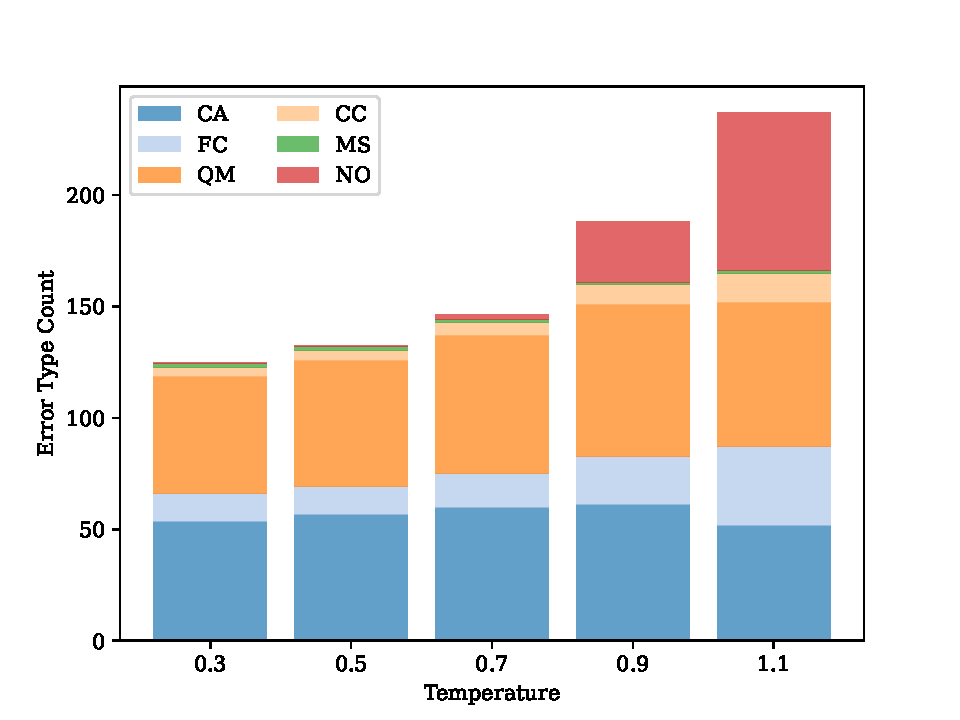
\includegraphics[width=0.8\textwidth]{figure/error_type_bar_math.pdf}
        \vspace{-1mm}
        \captionsetup{labelformat=empty}
        \addtocounter{figure}{-1}
        \caption{(a) Error type distribution on MATH. }
        \label{fig:error_type_bar}
    \end{minipage}        
    \hfill 
    \begin{minipage}{0.6\textwidth}
        \centering
        \small
        \begin{tcolorbox}[boxrule=0.5mm, left=1mm, right=1mm, top=1mm, bottom=1mm,
        fontupper=\scriptsize,
        fonttitle=\scriptsize,
        title=\textbf{Question:} What is $10.0000198 \cdot 5.9999985401 \cdot 6.9999852 $ to the nearest whole number?]
            \textbf{Answer (t=0.3)} First, we can multiply the first two numbers together: $10.0000198 \cdot 5.9999985401=59.9999999999$.  Then, we can multiply this number by the third number: $59.9999999999 \cdot 6.9999852=419.9999999999$.  Since this number is so close to $420$, we can round it to the nearest whole number, which is $\boxed{420}$.
            
            \textbf{Answer (t=0.9)} It is important to look closely and decide if the operation is really multiplication! Long ways of writing 5 or 10 could mean addition, so we need to pay attention so we don't fall into this common trap. And in this case, $(\text{Decimals}) \cdot (\text{Decimals}) = \text{Decimals}.$ ...
        \end{tcolorbox}
        \vspace{-4mm}
        \captionsetup{labelformat=empty}
        \addtocounter{figure}{-1}
        \caption{(b) An example of the generated reasoning trajectory at different sampling temperature.}
        \label{fig:error_type_case}
    \end{minipage}
    \caption{The shortcoming of sampling erroneous trajectories via increasing temerature: Using higher temperatue produces a substantial amount of nonsensical text, which is not observed in normal generation. Solutions are generated by \textit{LLaMA3-8B}.}
    \label{fig:high_temperature}
\end{figure*}
